\section{Extruding PLCL\label{methodology:extrudingPLCL}}

\subsection{Summary of PLCL Extrusions\label{methodology:extrudingPLCL:plclSummary}}

A significant portion of the research in this thesis pertains to extruding PLCL into a 3D printable filament. Multiple methods were employed to eventually achieve this. In summary, powder extrusions were first attempted. This was followed by manually and then automatically combining PLA and PCL pellets in a single screw extruder. Two extruders, 3Devo Filament Maker 1 and the Felfil Evo, were used to conduct these extrusions. Finally, shredding or regrinding the initial PLCL output and re-extruding was tested to address thickness tolerance concerns. Figure~\ref{methodology:extrudingPLCL:plclSummary} outlines this process at a high level.

\begin{figure}[h!]
        \centering
        \includegraphics[width=\linewidth]{../figs/methodology/plclExtrusions/plcl_extrusion_summary.png}
        \caption{Overview of the progression of PLCL extruding research.}
        \label{fig:methodology:extrudingPLCL:plclSummary}
\end{figure}

Additionally,~\fullref{tab:appendix:extrusionSummary} details all extrusions performed and their results.

\subsection{Powder Extrusions\label{sec:methodology:extrudingPLCL:powderExtrusion}}

Based on material availability, the team attempted to extrude PLCL powder to create PLCL filament. While pellets are more commonly extruded than powders (see~\fullref{sec:literatureReview:extrusion:powder}), the team was unable to source PLCL pellets at a scalable price. As a result, Nomisma PLCL powder was used~\cite{RefWorks:RefID:387-nomisma} for these initial extrusions on a 3Devo Filament Maker 1 single screw extruder.

Prior to extruding, the PLCL powder was dried in a vaccuum oven at 45\textcelsius ~overnight based on the material manufacturer's recommendations. The Polymer Synthesis Research Facility (PSRF) at Ohio State University was utilized for this task (see~\fullref{sec:methodology:externalLabs:polymersLab} for more information on research conducted with this additional lab).

The powder was measured and poured into the extruder as shown in Figure~\ref{fig:methodology:extrudingPLCL:powderExtrusion}.

\begin{figure}[h!]
        \centering
        \includegraphics[width=0.7\linewidth]{../figs/methodology/plclExtrusions/powderExtrusion/powder_extrusion.png}
        \caption{Performing PLCL powder extrusion. Measuring powder (left) and pouring into extruder (right).}
        \label{fig:methodology:extrudingPLCL:powderExtrusion}
\end{figure}

In addition to pouring the powder, a pusher inspired by the Devostick was employed~\cite{RefWorks:RefID:396-3devotroubleshooting}. This is a rectangular piece of wood used to compress the material in hopes of resolving feeding issues. Using the pusher piece is shown below in ~\autoref{fig:methodology:extrudingPLCL:devostick}.

\begin{figure}[h!]
        \centering
        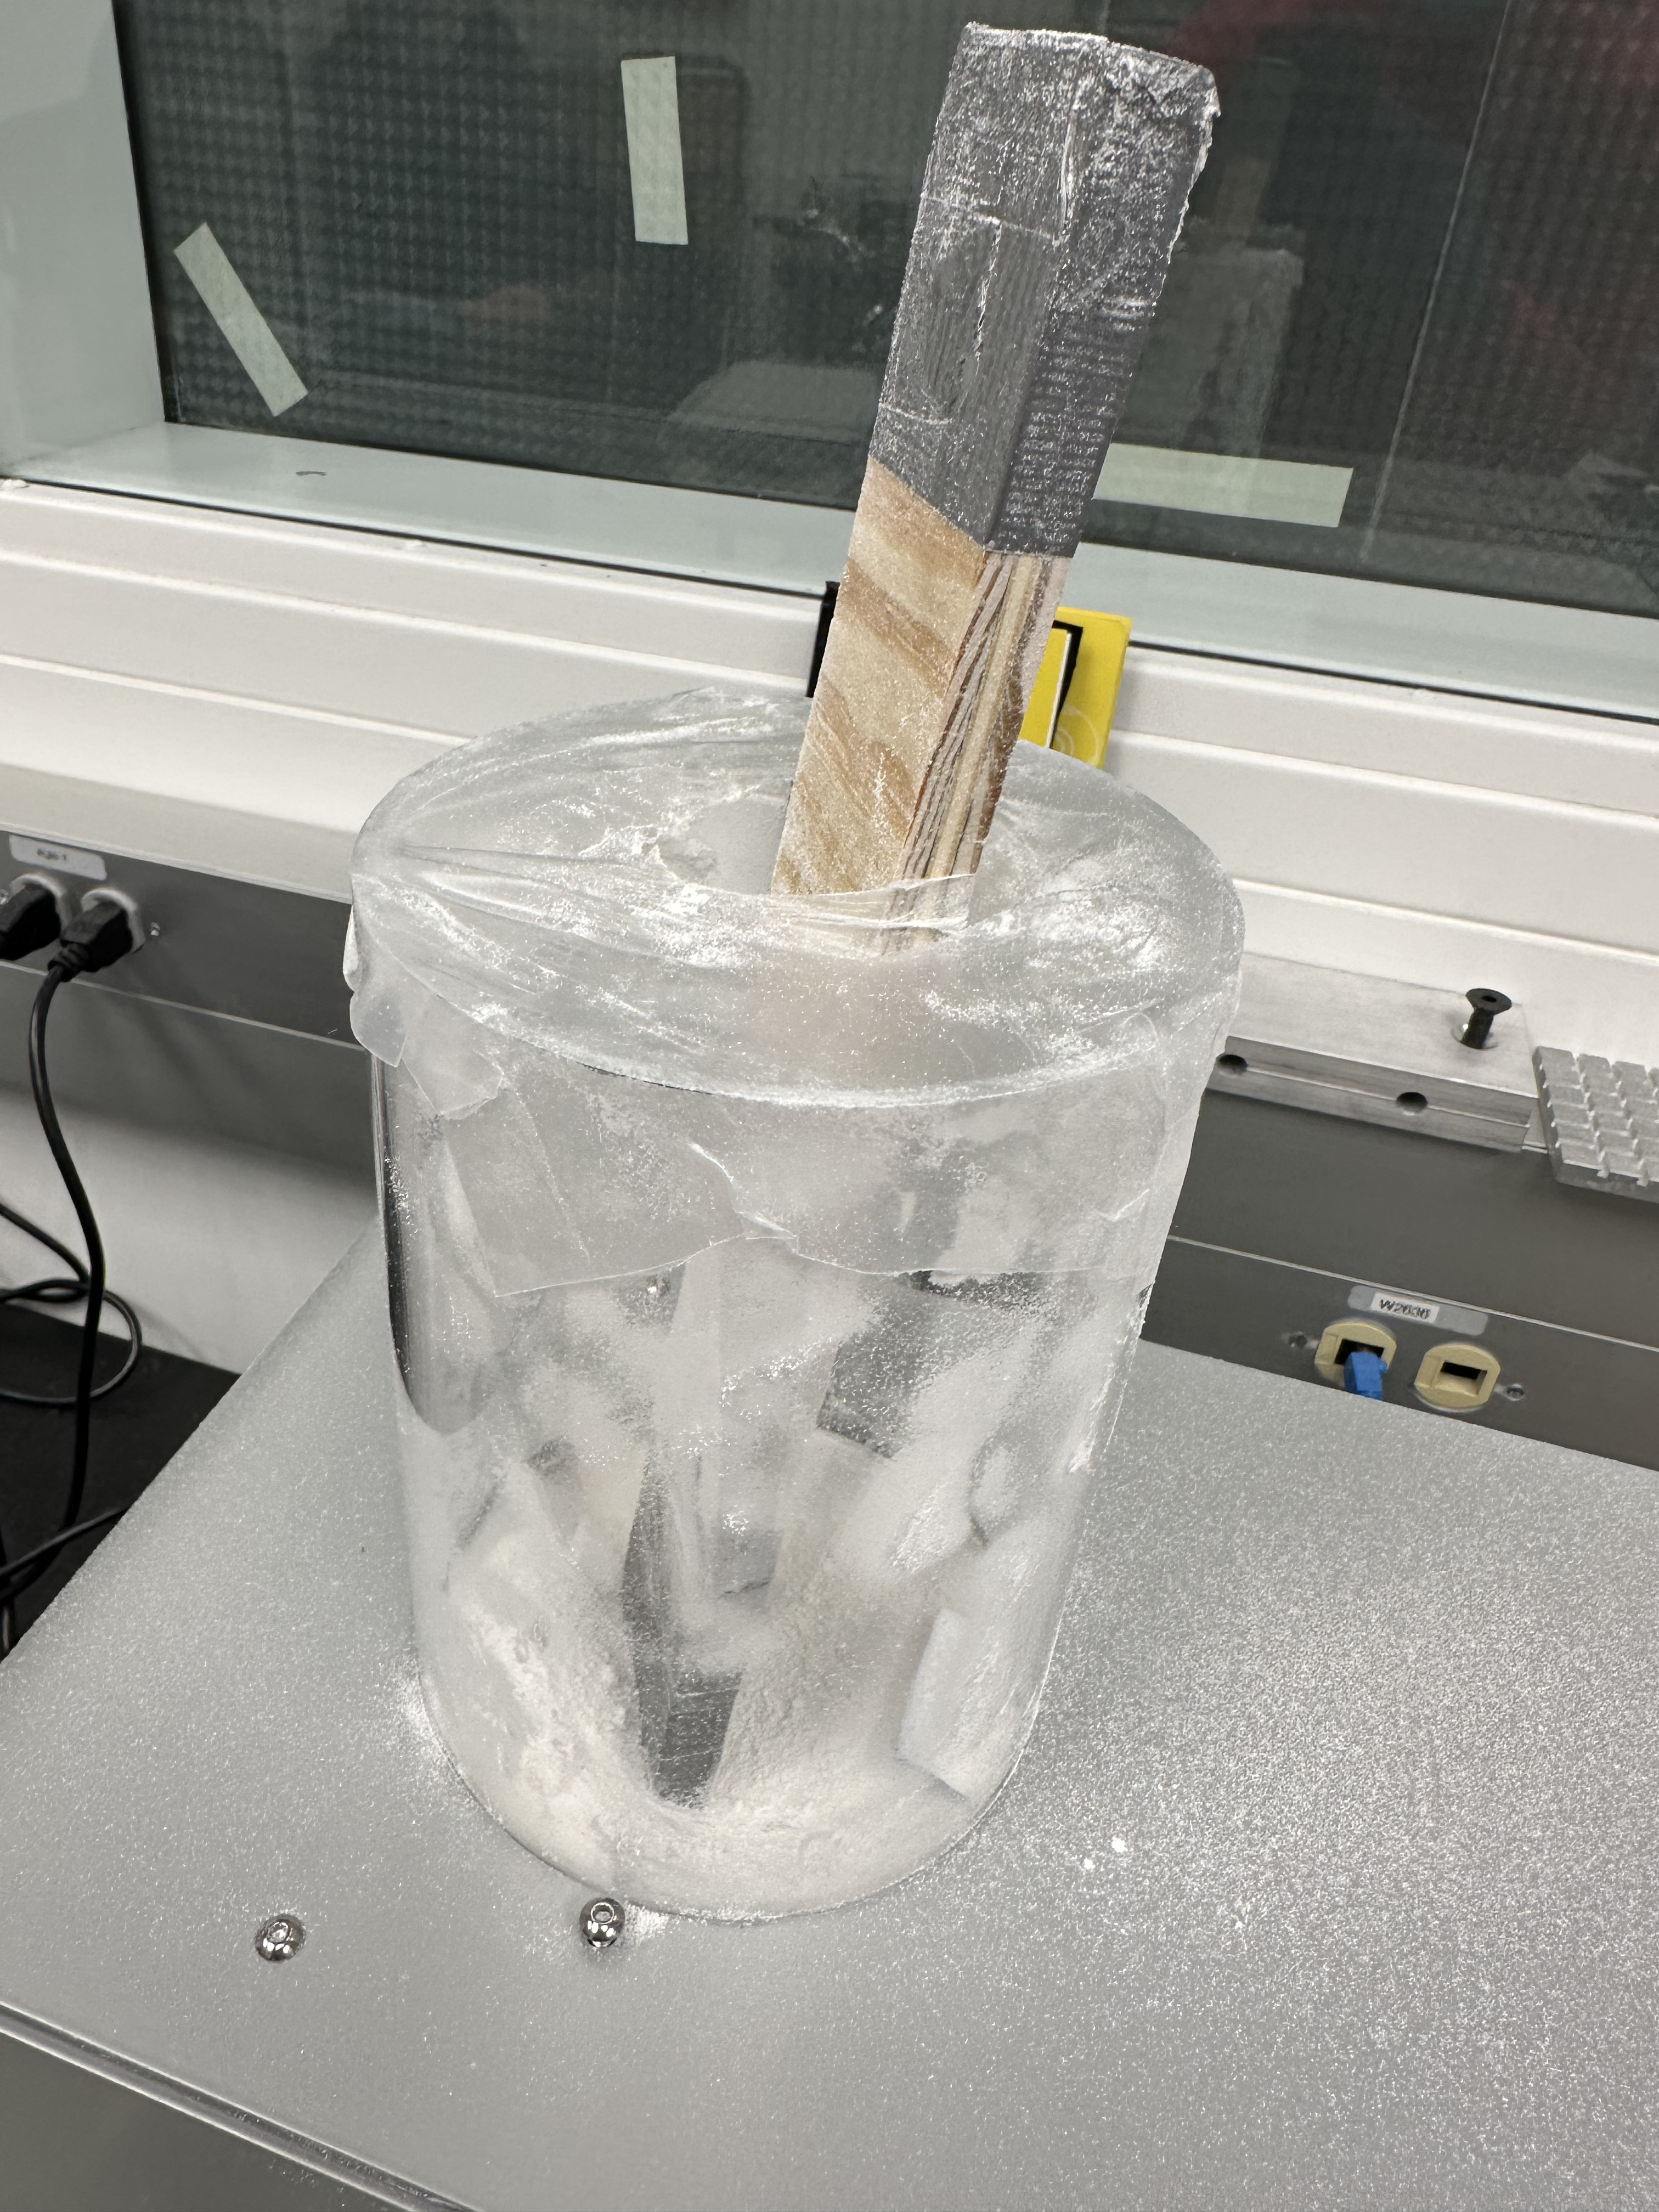
\includegraphics[width=0.5\linewidth]{../figs/methodology/plclExtrusions/powderExtrusion/devostick.png}
        \caption{Using the self-made "Devostick".}
        \label{fig:methodology:extrudingPLCL:devostick}
\end{figure}

This extruder has four heat zones with heater 4 (H4) being closest to the hopper and heater 1 (H1) being closest to the nozzle. Heaters 4 through 1 were set to 205\textcelsius, 200\textcelsius, 195\textcelsius, and 190\textcelsius ~respectively based on 3Devo customer support recommendations. The RPM for the extruder was set to 3.5.

To achieve these temperatures, the extruder was first run at PLA presets (H4-H1: 170, 185, 190, 170 (all in \textcelsius)). Temperatures were raised to HDPE presets (190\textcelsius ~across all heat zones) and HDPE was introduced into the extruder. Finally, temperatures were raised to the PLCL extruding temperatures and the PLCL powder was introduced into the extruder. DevoVision was used to monitor extruder parameters and variables such as current and heater temperatures.

The results and discussion for this experiment can be found in~\fullref{sec:results:extrudingPLCL:powderExtrusion} and~\fullref{sec:discussion:extrudingPLCL:powderExtrusion} respectively.

\subsection{Pellet Extrusions\label{sec:methodology:extrudingPLCL:pelletExtrusions}}
% Pivoted to pellets based on powder struggles and lit review
Based on the  difficulties and inherent brittleness of powder-based extrusions, the team explored relevant literature and decided to combine the copolymers of PLCL, PLA and PCL, in pellet form. This allows the extrusion to be completed with pellets rather than powder(s).

\subsubsection{Combining Raw Materials\label{sec:methodology:extrudingPLCL:pelletExtrusions:combiningMaterials}}
After deciding to explore pellet-based extrusions using PLA and PCL pellets, the team investigated how to best combine the two materials into a semi-homogenous mixture for extruding. Various methods the team explored were utilizing equipment with the College of Pharmacy, injection molding, chemically combining the two materials, mixing the materials in a tumbler, and discussing mixing concerns with extrusion subject-matter experts (SMEs) in the Department of Industrial Systems and Engineering at Ohio State University.~\fullref{sec:discussion:extrudingPLCL:pelletExtrusions:combiningMaterials} explains the findings of this investigation.

See~\fullref{sec:literatureReview:PLCL} for relevant literature on synthesizing PLCL.

\paragraph*{College of Pharmacy}
The team contacted the college of pharmacy at The Ohio State University due to the substantial mixing that occurs in pharmaceutical research. The team also toured the college of pharmacy's research facilities to better understand their equipment capabilities.

\paragraph*{Injection Molding}
The team also explored injection molding as a means of combining the PLA and PCL pellets. This was done by reviewing relevant literature and meeting with knowledgable professors at Ohio State University.

\paragraph*{Chemically Combining Materials}
Following existing literature, the team explored chemically combining PLA and PCL such as by dissolving the materials in dichloromethane (DCM) or chloroform.

The team also evaluated melting the pellets together on a hotplate with a magnetic and manual stirrer as shown below in~\autoref{fig:methodology:extrudingPLCL:meltingOnHotplate}

\begin{figure}[h!]
        \centering
        \includegraphics[width=0.5\linewidth]{../figs/methodology/plclExtrusions/pelletExtrusions/combining_on_hotplate.png}
        \caption{Melting PLA and PCL using a hotplate with mixing (left) and final output (right).}
        \label{fig:methodology:extrudingPLCL:meltingOnHotplate}
\end{figure}

\paragraph*{3D Printable Mixing Systems}

Mixing the pellets in a tumbler styler mixer was also explored. To lower the cost and development time, 3D printing a mixing system was explored. Various premade models of rotary tumbler mixers were found through online CAD repositories such as Thingiverse. Examples of 3D printable mixers are shown in Figure~\ref{fig:methodology:extrudingPLCL:3dPrintableMixers}

\begin{figure}[h!]
        \centering
        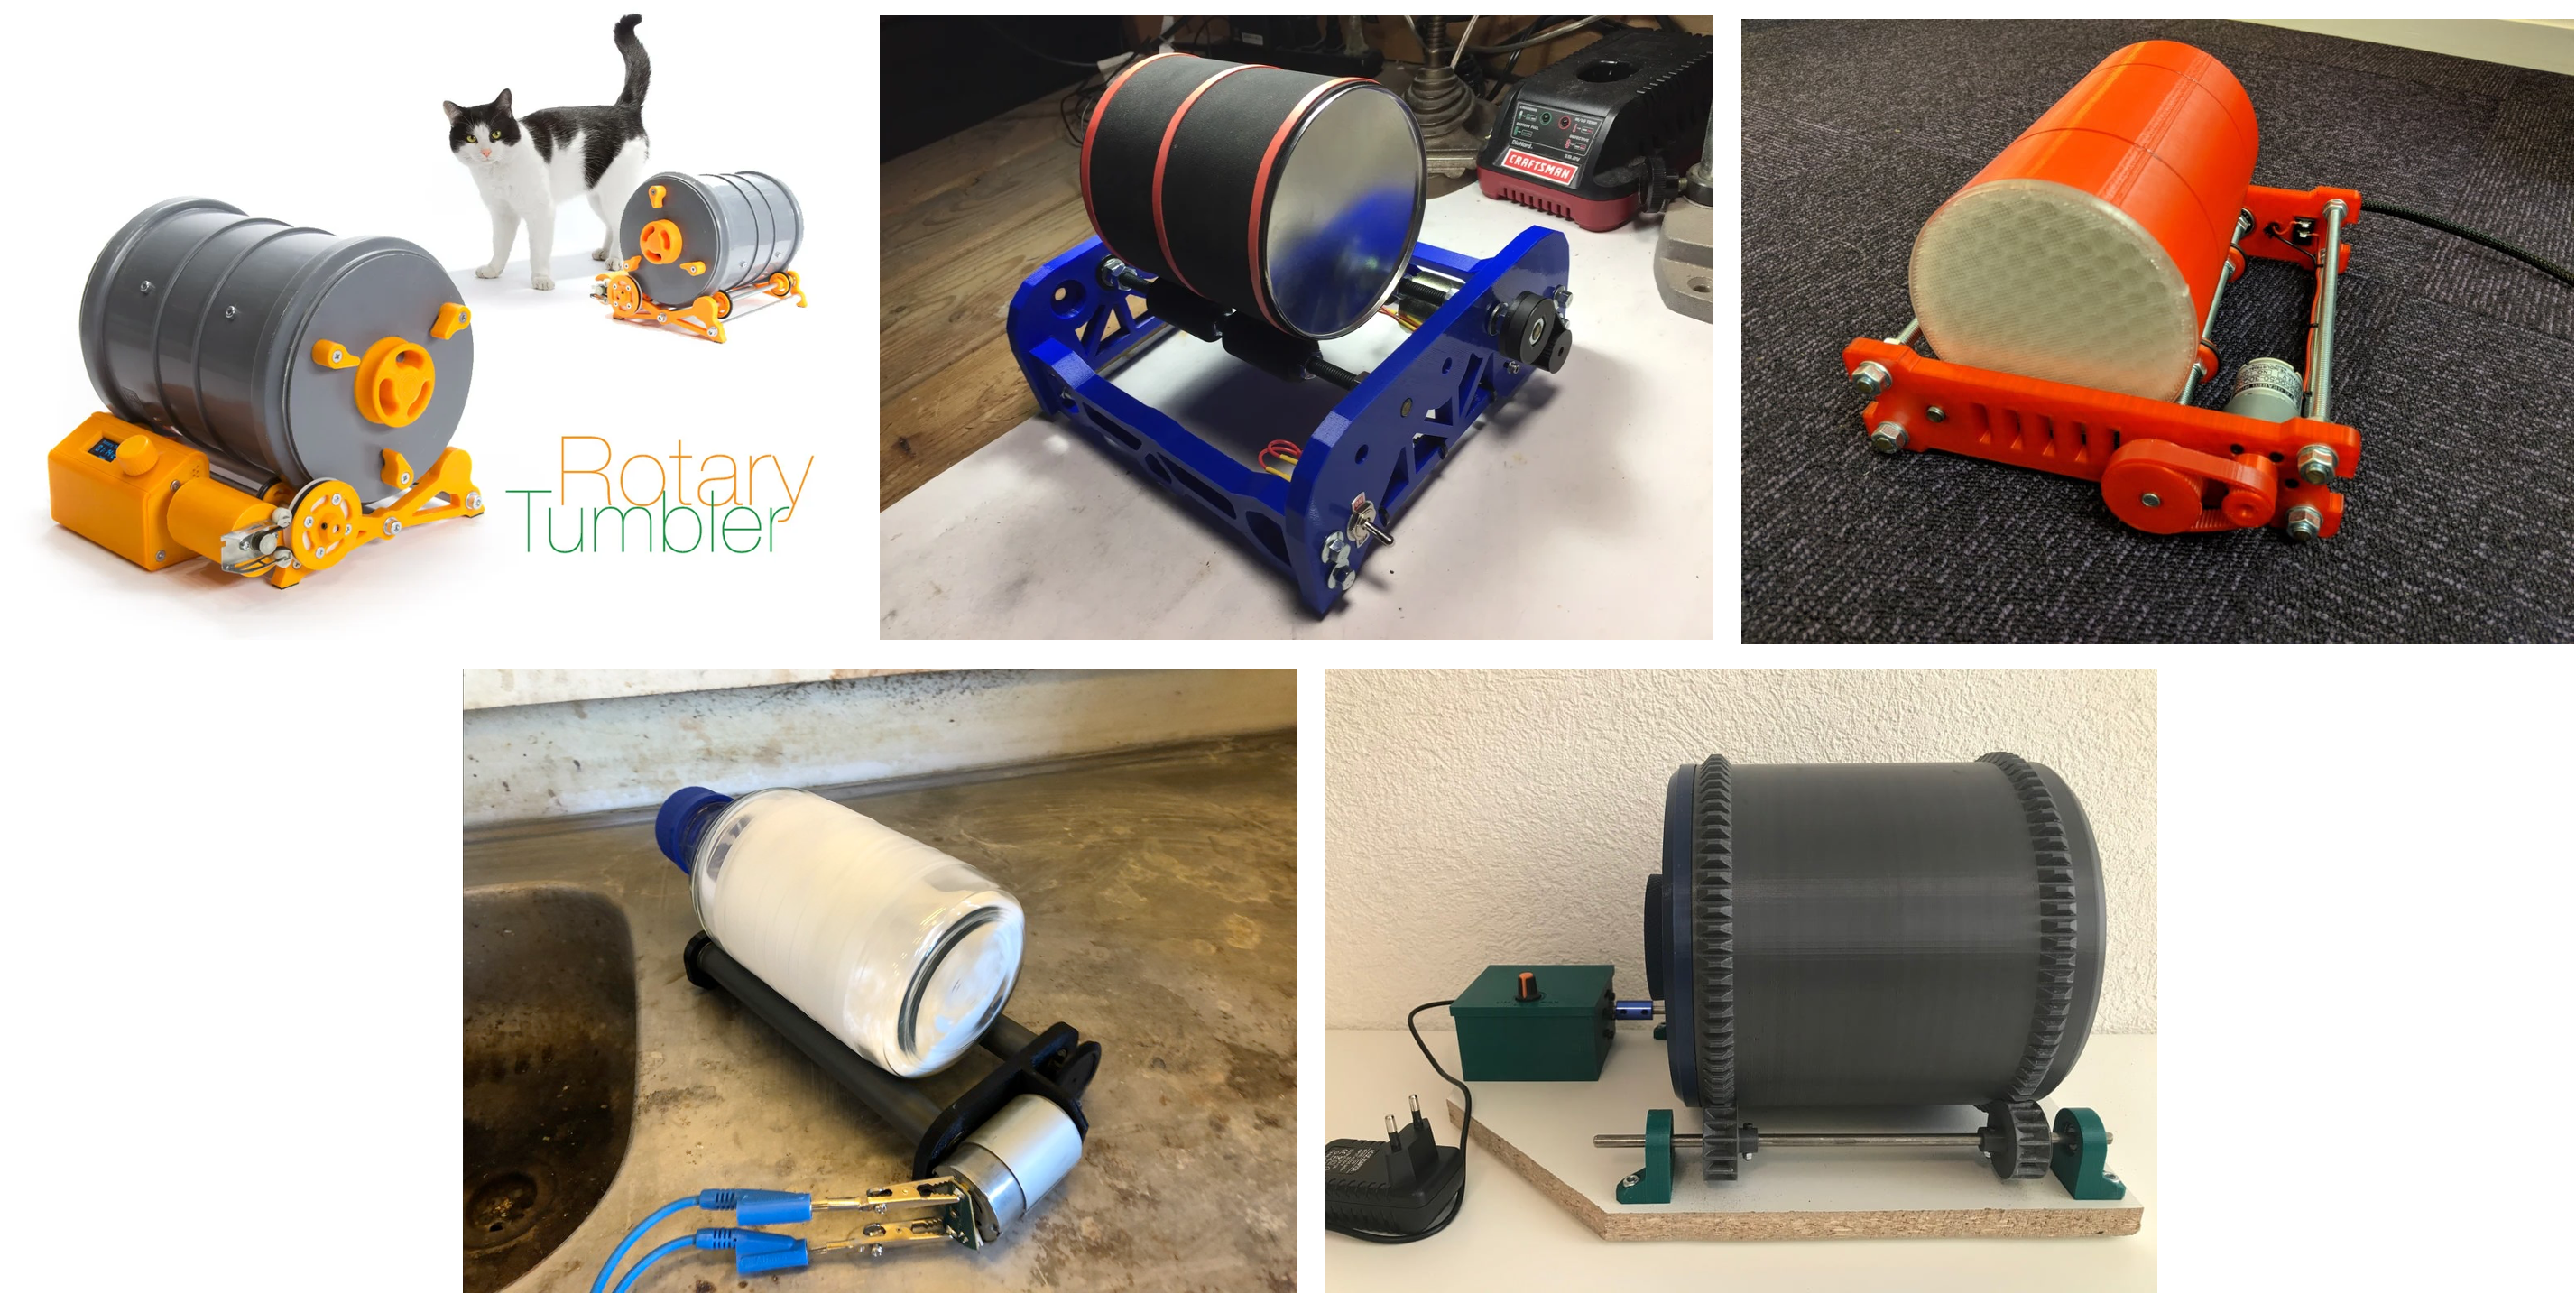
\includegraphics[width=0.7\linewidth]{../figs/methodology/plclExtrusions/pelletExtrusions/3d_printed_mixers.png}
        \caption{Various 3D printable tumbler mixers~\cite{RefWorks:RefID:482-lucasfrit2021ball,RefWorks:RefID:483-bluepop42017rock,RefWorks:RefID:484-dariocarioli2018rotary,RefWorks:RefID:485-jonathanlundstrom2018simple,RefWorks:RefID:486-perinski2018rotary}.}
        \label{fig:methodology:extrudingPLCL:3dPrintableMixers}
\end{figure}

\paragraph*{Discussions with ISE Department}
The team also met with extrusion subject-matter experts in the Industrial and Systems Engineering (ISE) department at The Ohio State University. This included Dr. Rachmat Mulyana.

\subsection{Initial Pellet Extrusion\label{sec:methodology:extrudingPLCL:pelletExtrusions:initialExtrusion}}

PLA pellets were purchased from 3DXTECH and PCL pellets were ordered from Sigma Aldrich~\cite{RefWorks:RefID:487-ecomax,RefWorks:RefID:488-polycaprolactone}. Following manufacturer recommendations, PLA and PCL pellets were dried overnight in a vacuum oven at 55\textcelsius and 40\textcelsius respectively prior to extruding.

After deciding to combine PLA and PCL pellets manually in a jar (see~\fullref{sec:discussion:extrudingPLCL:pelletExtrusions:combiningMaterials}), an initial pellet extrusion was performed.

Figure~\ref{fig:methodology:extrudingPLCL:mixingPellets} shows the pellet mixture before and after mixing. The white colored pellets are PCL and the tan colored pellets are PLA. A 70/30 mixture of PLA/PCL was created by weight with roughly 70g of PLA and 30g of PCL.

\begin{figure}[h!]
        \centering
        \includegraphics[width=0.7\linewidth]{../figs/methodology/plclExtrusions/pelletExtrusions/mixing_pellets_manually.png}
        \caption{Mixing pellets manually. Unmixed (left), mixed (middle and right).}
        \label{fig:methodology:extrudingPLCL:mixingPellets}
\end{figure}

In this extrusion, the 3Devo Feeder was used for the first time. The temperature profile was is shown below in Table~\ref{tab:methodology:extrudingPLCL:initialPelletExtrusion:tempPresets} based on existing literature~\cite{RefWorks:RefID:253-åkerlund2022effect}. All pellets were poured into the hopper with the Feeder running and the extrusion began.

\begin{table}[h!]
        \centering
        \caption{Initial pellet extrusion temperature presets\label{tab:methodology:extrudingPLCL:initialPelletExtrusion:tempPresets}}
        \begin{tabular}{l c}
                \hline
                \textbf{Heater} & \textbf{Temperature (\textcelsius)} \\
                \hline
                H4              & 140                                 \\
                H3              & 155                                 \\
                H2              & 160                                 \\
                H1              & 160                                 \\
                \hline
        \end{tabular}
\end{table}

Results and discussion of this extrusion can be found in ~\fullref{sec:results:extrudingPLCL:pelletExtrusions:initialPelletExtrusion} and ~\fullref{sec:discussion:extrudingPLCL:pelletExtrusions:initialPelletExtrusion} respectively.

\subsection{PCL Temperature Study\label{sec:methodology:extrudingPLCL:pelletExtrusions:pclExtrusions}}
% Extruded just PCL to find extrudable temp and make sure it overlapped with PLA
% Found starve feeding helps with melting in the hopper
% Inspired to develop automatic starve feeder

Based on findings from the initial pellet extrusion (see~\fullref{sec:discussion:extrudingPLCL:pelletExtrusions:initialPelletExtrusion}), a study was performed to determine the working extrusion temperature of PCL pellets. A PCL extrusion process developed by 3Devo was followed which first involved  extruding PLA pellets at normal presets. All heaters were then set to 170\textcelsius ~and PCL was introduced. Once the filament output had shifted from PLA to PCL, which is apparent based on the filament color being white rather than clear, the temperature of all heaters was lowered to 60\textcelsius. From here, the temperature was raised in increments of 10\textcelsius ~to determine how high of a temperature PCL could be easily extruded at~\cite{RefWorks:RefID:489-3devo2024extrusion}.

Based on time available, this extrusion was divided into two sequential extrusions. The first tested PCL between 60\textcelsius ~and 110\textcelsius ~while the second extrusion tested PCL between 120\textcelsius ~and 180\textcelsius.

Starve feeding was also explored during these extrusions. Extrusion 1 (60-110\textcelsius) employed manual starve feeding. An Excel spreadsheet was used to track the amount of PCL poured and the time between pours. A section of that spreadsheet is shown below in Figure~\ref{fig:methodology:extrudingPLCL:manualStarveFeedingLog}.

\begin{figure}[h!]
        \centering
        \includegraphics[width=\linewidth]{../figs/methodology/plclExtrusions/pelletExtrusions/manual_starve_feeding_log.png}
        \caption{Section of manual starve feeding Excel spreadsheet.}
        \label{fig:methodology:extrudingPLCL:manualStarveFeedingLog}
\end{figure}

Results and discussion of the PCL temperature study can be found in ~\fullref{sec:results:extrudingPLCL:pelletExtrusions:pclTempStudy} and ~\fullref{sec:discussion:extrudingPLCL:pelletExtrusions:pclTempStudy} respectively. Results and discussion of the manual starve feeding can be found in ~\fullref{sec:results:extrudingPLCL:pelletExtrusions:manualStarveFeeding} and ~\fullref{sec:discussion:extrudingPLCL:pelletExtrusions:manualStarveFeeding} respectively.

\subsection{Starve Feeding Based Pellet Extrusions\label{sec:methodology:extrudingPLCL:pelletExtrusions:usingStarveFeeder}}
% Finally successful but too thin
% Shredding and re-extruding looked promising (using extruder to combine pellets initially) but still led to variable flow rate due to regrind
Based on the repetitive and exact nature of the manual starve feeding, an automatic starve feeder was developed (see ~\fullref{sec:discussion:extrudingPLCL:pelletExtrusions:manualStarveFeeding} for more details on this decision). This development is detailed in ~\fullref{sec:methodology:starveFeeder}.

The starve feeder was first tested on PCL during the second temperature test extrusion from 120\textcelsius ~to 180\textcelsius. Once it was proven to work, the starve feeder was used on a PLCL extrusion.

\subsubsection{Initial PLCL Extrusion with Starve Feeder\label{sec:methodology:extrudingPLCL:pelletExtrusions:usingStarveFeeder:initialPLCLExtrusion}}

With the new starve feeder (see ~\fullref{sec:methodology:starveFeeder}), a second pellet-based PLCL extrusion was attempted using a 70/30 blend of PLA and PCL pellets.

The extrusion began with just PLA pellets at 180\textcelsius. Once this was extruding well, a 70/30 blend of PLA and PCL pellets was introduced using the starve feeder. Once the output transitioned to PLCL, the temperature was lowered from 180\textcelsius ~to 160\textcelsius ~in 5 degree increments to approach the preferred extrusion temperature for PCL (see~\fullref{sec:results:extrudingPLCL:pelletExtrusions:pclTempStudy}).

The filament output was then spooled by feeding the output through the filament sensor and into the spooler on the 3Devo Filament Maker One. Filament thickness was variable and on average too low (1.4mm instead of 1.75mm). Various parameters were adjusted to try and improve the filament thickness average and consistency. Overall, the thickness was not able to be improved, and the extrusion was terminated by extruding solely PLA pellets.

The highlights of this extrusion can be found below in Table.

\begin{table}[h!]
        \centering
        \caption{Extrusion process conditions and observations.}
        \label{methodology:extrudingPLCL:pelletExtrusions:usingStarveFeeder:initialPLCLExtrusion}
        \begin{adjustbox}{max width=\textwidth}
                \begin{tabular}{l c c c c l}
                        \hline
                        \textbf{Time (HH:MM:SS)} & \textbf{Heater Temp (\textcelsius)} & \textbf{Pellet Rate (g/s)} & \textbf{Material} & \textbf{Quality} & \textbf{Notes}                                  \\
                        \hline
                        0{:}00{:}22              & 180                                 & N/A                        & PLA               & Good             & Extruding PLA                                   \\
                        0{:}26{:}40              & 180                                 & 2/80                       & PLA/PCL           & Good             & Started Extruding PLA/PCL Blend                 \\
                        1{:}00{:}00              & 170                                 & 2/80                       & PLA/PCL           & Good             &                                                 \\
                        1{:}22{:}10              & 165                                 & 2/100                      & PLA/PCL           & Good             &                                                 \\
                        1{:}43{:}20              & 160                                 & 2/100                      & PLA/PCL           & Good             &                                                 \\
                        2{:}05{:}30              & 160                                 & 2/100                      & PLA/PCL           & Good             & Started Spooling Output                         \\
                        2{:}15{:}00              & 165                                 & 1/100                      & PLA/PCL           & Thin             & Filament thickness too thin (1.4 mm)            \\
                        2{:}36{:}40              & 165                                 & 1/100                      & PLA/PCL           & Thin             & Tried Increasing RPM to Address Thickness       \\
                        2{:}53{:}45              & 165                                 & 1/60                       & PLA/PCL           & Thin             & Tried Increasing Pour Rate to Address Thickness \\
                        3{:}30{:}00              & 170                                 & N/A                        & PLA               & Good             & Ended Extrusion                                 \\
                        \hline
                \end{tabular}
        \end{adjustbox}
\end{table}

Results and discussion of this initial starve-feeder based PLCL extrusion can be found in ~\fullref{sec:results:extrudingPLCL:pelletExtrusions:initialStarveFeederExtrusion} and ~\fullref{sec:discussion:extrudingPLCL:pelletEtrusions:initialStarveFeederExtrusion} respectively.

\subsubsection{Addressing Filament Thickness\label{sec:methodology:extrudingPLCL:pelletExtrusions:usingStarveFeeder:addressingFilamentThickness}}

After performing a Devo Mid-Temp (MT) purge (see ~\fullref{sec:methodology:extrudingPLCL:purgingExtruder}), multiple other PLCL pellet-based extrusion were attempted as detailed in ~\autoref{tab:appendix:extrusionSummary}.

\paragraph*{Adjusting Heat Zones}

Following recommendations from 3Devo customer support, the temperature of heater 4 was lowered to 100\textcelsius ~which was as low as it could get. The goal was with this lower initial heat, more solidified material would be pushing the softer material through the rest of the barrel.

Eventually extrusions were attempted with heater 4 and heater 3 at 100\textcelsius. Additionally, the RPM was raised incrementally from 3.5 to 7 to see if this parameter helped address filament thickness.

A final extrusion was attempted following a published methodology that used a 3Devo Filament Maker One but pre-combined PLA/PCL pellets. This paper set heat zones to 140, 155, 160, and 160 (all \textcelsius) for heaters four through 1 respectively~\cite{RefWorks:RefID:253-åkerlund2022effect}.

Results and discussion of this heat zone adjustment research can be found in ~\fullref{sec:results:extrudingPLCL:pelletExtrusions:addressingFilamentThickness} and ~\fullref{sec:discussion:extrudingPLCL:pelletExtrusions:addressingFilamentThickness} respectively.

\paragraph*{Extruding PLCL Regrind}

Many papers that successfully extruded PLCL using PLA and PCl pellets combined the material beforehand (see ~\fullref{sec:literatureReview:PLCL}). While research was conducted on combining PLA and PCL prior to extruding (see ~\fullref{sec:methodology:extrudingPLCL:pelletExtrusions:combiningMaterials}), many of these options were unable to be performed by the research team.

After failing to resolve the filament thickness variability, however, the idea of combinging PLA and PCL prior to extrusion was revisited. As a result, in a similar manner to injection molding, it was hypothesized that re-extruding the initial filament output (which had been thermally combined during the first pass through the extruder) may behave similar to existing literature. To test this, initial filament output, referred to as first-pass PLCL, was shredded using a Felfill Shredder+ and re-extruded through the 3Devo Filament Maker One. The process of creating PLCL regrind to extrude is illustrated below in Figure~\ref{fig:methodology:extrudingPLCL:pelletExtrusions:creatingRegrind}.

\begin{figure}[h!]
        \centering
        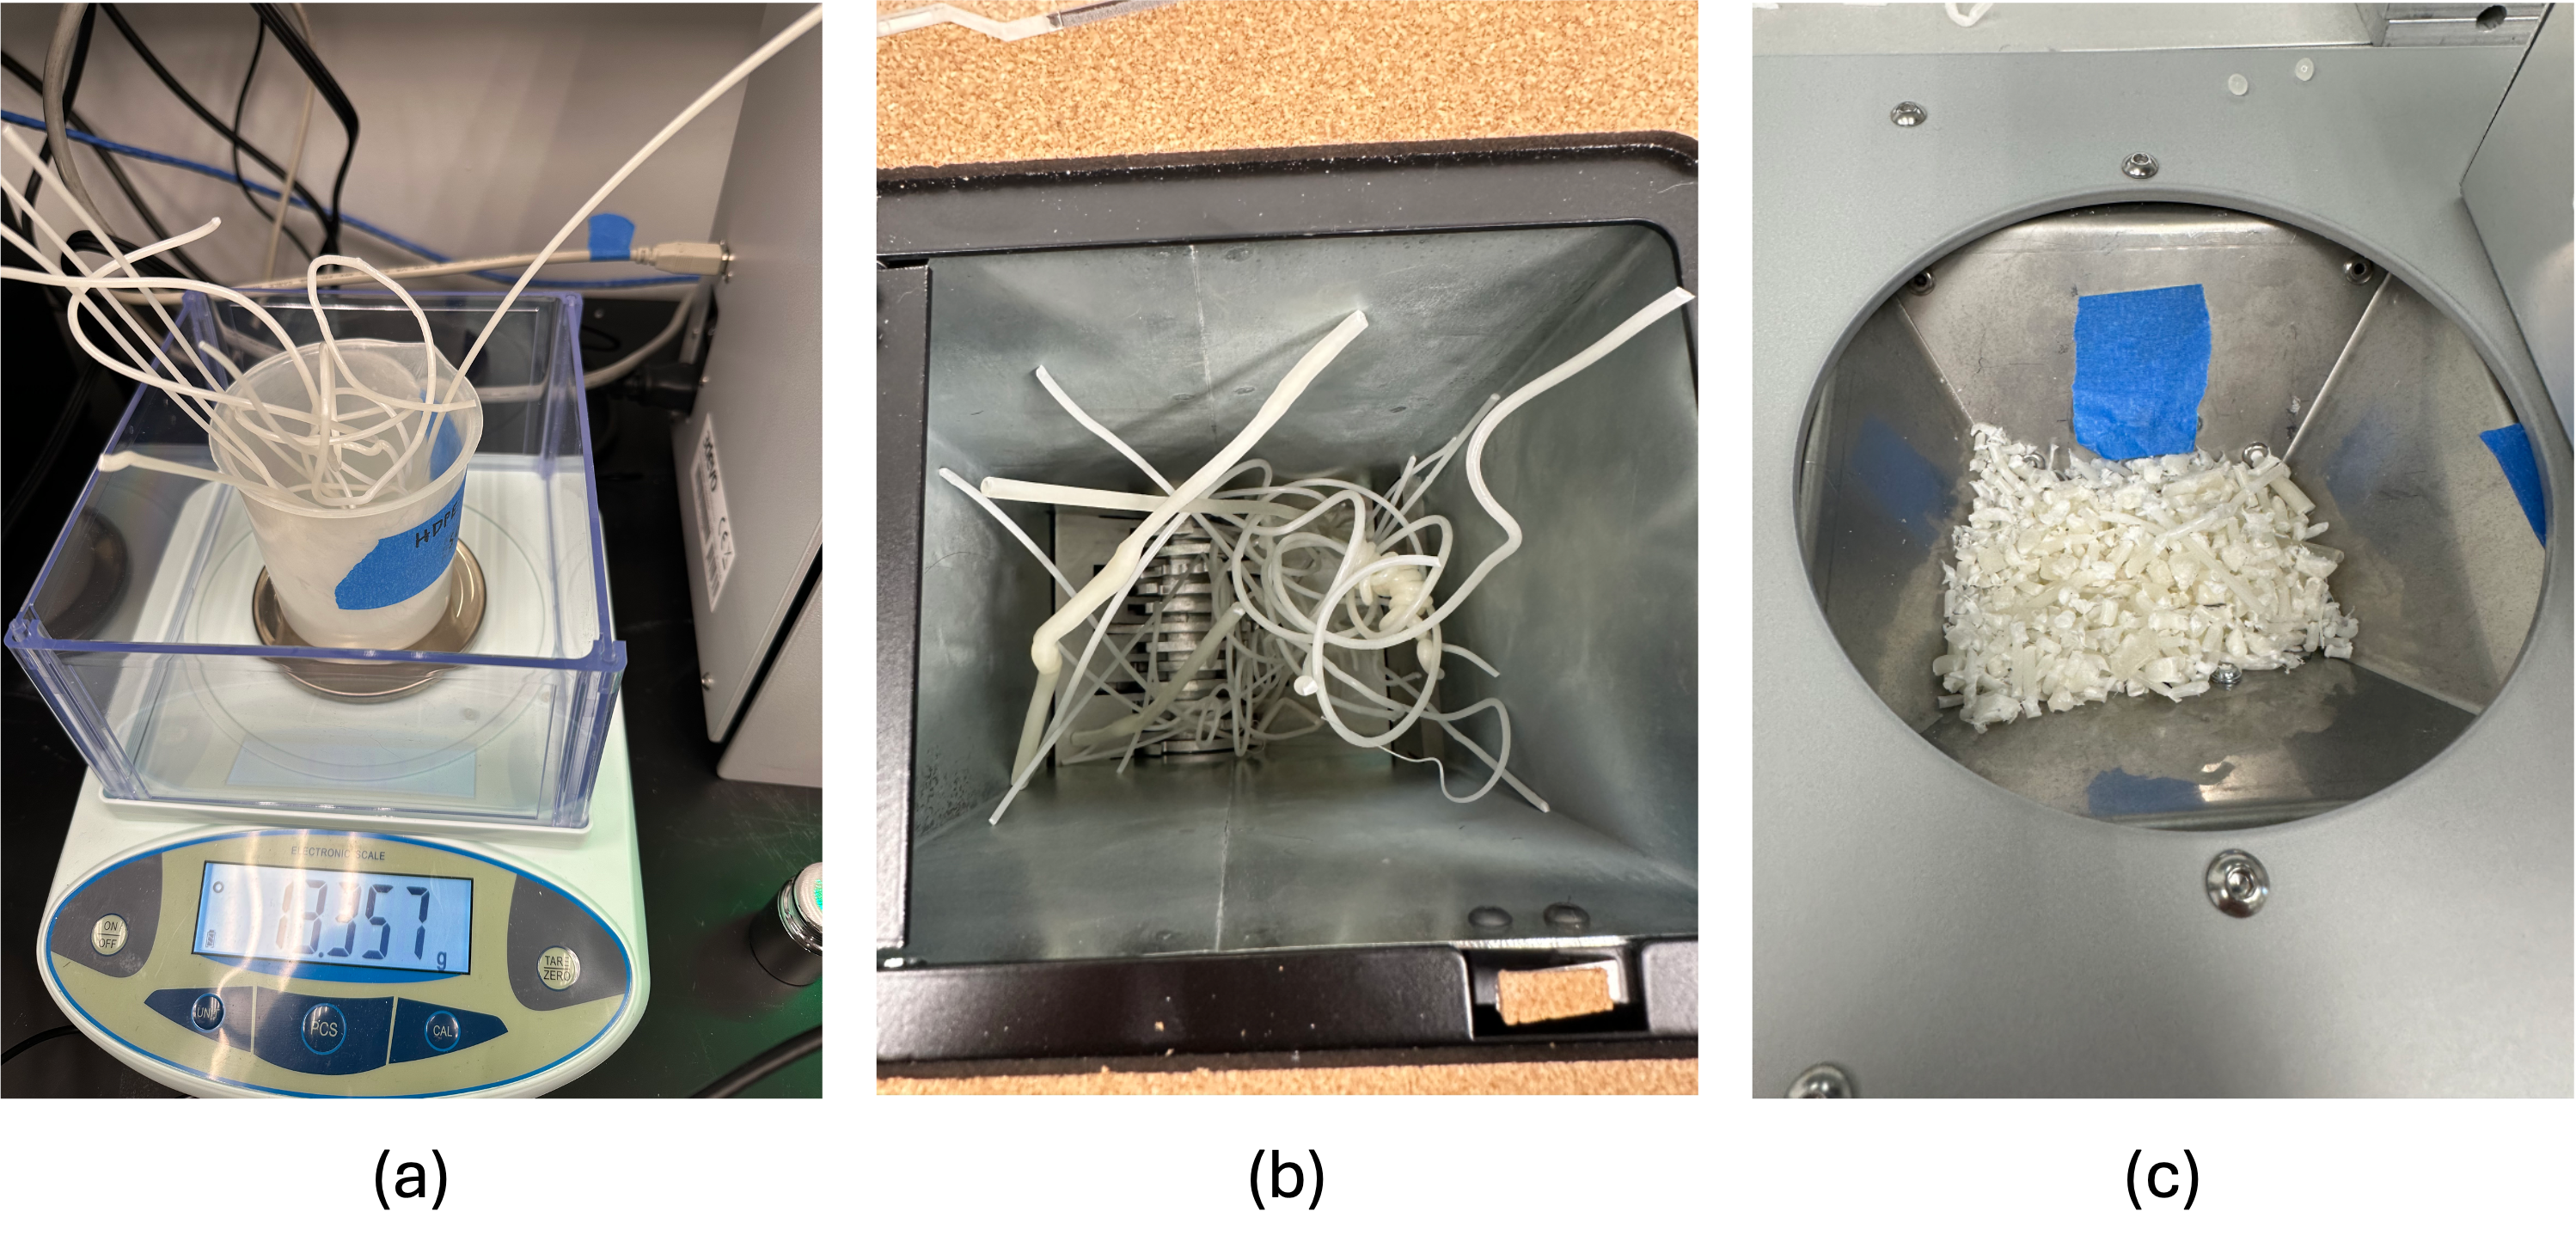
\includegraphics[width=\linewidth]{../figs/methodology/plclExtrusions/pelletExtrusions/extruding_plcl_regrind_process.png}
        \caption{Process of creating PLCL regrind. (A) Weighing 1st pass PLCL, (B) Shredding 1st pass PLCL, (C) Pouring regrind into hopper.}
        \label{fig:methodology:extrudingPLCL:pelletExtrusions:creatingRegrind}
\end{figure}

Results and discussion of this re-extrusion research can be found in ~\fullref{sec:results:extrudingPLCL:pelletExtrusions:addressingFilamentThickness} and ~\fullref{sec:discussion:extrudingPLCL:pelletExtrusions:addressingFilamentThickness} respectively.

\paragraph*{Clogged Extruder}

It was also noticed that routinely while transitioning from low heater 4 and heater 3 back to PLA presets, a clog often formed in the machine. Due to a limited supply of purging compound, PLA was used to push out the PLA/PCL clog which usually required running the extruder for an hour.

\subsection{Purging 3Devo Extruder\label{sec:methodology:extrudingPLCL:purgingExtruder}}
% iii.	Purging Compounds
% 1.	Found initial supplier of 3Devo DevoClean Mid-Temp
% 2.	Worked with supplier (Dyna-Purge) to find ideal purging material
% a.	Tried L then D2 (needs HDPE) then K

Following clogging and overly thin filament output (see ~\fullref{{sec:methodology:extrudingPLCL:pelletExtrusions:usingStarveFeeder:addressingFilamentThickness}}), purging the extruder was further researched.

\subsubsection{Initial Purging Process\label{sec:methodology:extrudingPLCL:purgingExtruder:initialProcess}}

Initially, the purging process followed was provided by 3Devo~\cite{RefWorks:RefID:405-purging}. This required DevoClean Mid-Temp (MT) and to transition from PLA/PCL to DevoClean MT and back. 1 kg of DevoClean MT was provided with the extruder purchase, but this material supply was becoming limited. As a result, purges were limited in an effort to preserve resources. This process is outlined below in Figure~\ref{fig:methodology:extrudingPLCL:purgingExtruder:3DevoProcess}

\begin{figure}[h!]
        \centering
        \includegraphics[width=\linewidth]{../figs/methodology/plclExtrusions/purgingExtruder/3devo_purge_overview.png}
        \caption{Overview of 3Devo DevoClean MT purging process~\cite{RefWorks:RefID:405-purging}.}
        \label{fig:methodology:extrudingPLCL:purgingExtruder:3DevoProcess}
\end{figure}

Results and discussion of the initial purging process can be found below in ~\fullref{sec:results:extrudingPLCL:pelletExtrusions:purgingExtruder:initialPurge} and ~\fullref{sec:discussion:extrudingPLCL:pelletExtrusions:purgingExtruder:initialPurge} respectively.

\subsubsection{Supplier Discovery\label{sec:methodology:extrudingPLCL:purgingExtruder:supplierDiscovery}}

The team reached out to 3Devo customer support directly to see DevoClean MT's technical data sheet (TDS) to better understand the material characteristics that should be matched in a replacement extruding compound. This TDS, however, was from a separate company, Dyna-Purge. Dyna-Purge is a company that specializes in extrusion compounds and is based in the United States.

The research team reached out to Dyna-Purge directly as buying from them would avoid international shipping that results from placing an order with 3Devo as they are based in the Netherlands.

\subsubsection{Dyna-Purge Collaboration\label{sec:methodology:extrudingPLCL:purgingExtruder:dynaPurgeCollaboration}}

According to Dyna-Purge, the DevoClean MT was a legacy product and has since been improved. Based on the melt flow index (MFI) of the extruded materials, multiple extruding compounds were suggested and two $10lb$ samples were sent from Dyna-Purge.

Dyna-Purge (abbreviated as DP) sent samples of their DP-D2 and DP-L extruding compounds. DP-D2 had an MFI similar to PCL whereas DP-L had an MFI similar to PLA. A similar MFI is necessary for properly pushing out existing material and effectively purging the extruder~\cite{RefWorks:RefID:493-gate}. DP-D2, required HDPE to transition materials, similar to DevoClean MT, which is unideal given the time and additional material required to perform a purge. A summary of these compounds is shown below in Table~\ref{tab:methodology:extrudingPLCL:dpCollaboration:comparingPurgingCompounds}.

\begin{table}[h!]
        \centering
        \caption{Summary of Dyna-Purge Purging Compounds.}
        \label{tab:methodology:extrudingPLCL:dpCollaboration:comparingPurgingCompounds}
        \begin{tabular}{l l c}
                \hline
                \textbf{Purging Compound} & \textbf{Ideal Material} & \textbf{Requires HDPE?} \\
                \hline
                DP-D2                     & PLA                     & Yes                     \\
                DP-L                      & PCL                     & No                      \\
                \hline
        \end{tabular}
\end{table}

\subsubsection{Purging with DP-L\label{sec:methodology:extrudingPLCL:purgingExtruder:dpLPurge}}

Initially, based on not requiring HDPE, DP-L was tested for purging the extruder. The purging process provided by Dyna-Purge was followed as outlined below in List~\ref{list:test}.

\begin{enumerate}
        \label{list:test}
        \item Finish extruding material
        \item Transition to purging compound
        \item Raise temperature (180\textcelsius ~to 250\textcelsius)
        \item Purge material while switching between high and low RPM
        \item Leave purging compound in barrel and start machine with a new purge
\end{enumerate}

This process is different from using DevoClean MT (see \autoref{fig:methodology:extrudingPLCL:purgingExtruder:3DevoProcess}) which suggests ending with the initial material rather than the purging compound inside the barrel.

Discussion of purging with DP-L can be found in ~\autoref{sec:discussion:extrudingPLCL:pelletExtrusions:purgingExtruder:dpLPurge}.

\subsubsection{Purging with DP-D2\label{sec:methodology:extrudingPLCL:purgingExtruder:dpD2Purge}}

Based on contamination following DP-L purges (see Section ~\ref{sec:discussion:extrudingPLCL:pelletExtrusions:purgingExtruder:dpLPurge}), DP-D2 was tested as a purging compound.

This material required HDPE to transition between PLA/PCL and DP-D2. Extrusion labs across The Ohio State University were contacted regarding extra HDPE that could be used. No labs were able to provide HDPE so $5lbs$ of HDPE pellets were ordered from McMaster-Carr~\cite{RefWorks:RefID:494-moistureresistant}.

The DP-D2 was used in purging identically to DP-L following Dyna-Purge's recommendations. Discussion of the DP-D2 purge testing can be found in Section~\ref{sec:discussion:extrudingPLCL:pelletExtrusions:purgingExtruder:dpD2Purge}.

\subsection{Felfil System\label{sec:methodology:extrudingPLCL:felfilSystem}}

Based on the thin filament output by the 3Devo Filament Maker One when extruding a PLA/PCL blend (see ~\ref{sec:methodology:extrudingPLCL:pelletExtrusions:usingStarveFeeder:addressingFilamentThickness}), the Felfil Evo was tested for PLCL extrusions.

The Felfil Evo had been used initially for powder-based PLCL extrusions, but research was paused due to unsuccessful results (see ~\ref{sec:introduction:priorWork:otherTeamWork:plclExtrusions}). Since the 3Devo Filament Maker One, a more robust extruder, also was unsuccessful extruding powders, it was hypothesized that powder-based extrusions for any extruder may be challenging and the Felfil Evo may be more effective with pellet-based extrusions.

\subsubsection{Felfil Evo Initial Testing\label{sec:methodology:extrudingPLCL:felfilSystem:felfilEvoInitialTesting}}

\paragraph*{Initial Repairs}

To begin testing the Felfil Evo, all remaining PLCL powder from prior research was cleaned using wipes and a vaccuum. The plastic hopper could not be fully cleaned, however, so a new hopper was 3D printed as a replacement. In an effort to save time, only the screws holding the hopper in place were removed rather than disassembling the entire hopper.

This overly simplistic disassembly led to a screw not being properly tightened and the barrel of the extruder was improperly secured to the hopper. When testing the extruder following this hopper replacement, the barrel, which should remain stationary, began rotating which led to a gap between the barrel and hopper. This gap is shown below in Figure~\ref{fig:methodology:extrudingPLCL:pelletExtrusions:felfilEvo:initialGap}.

This gap allowed material to fall when traveling from the hopper to the barrel and also negatively impacted the overall insulation of the extruder.

\begin{figure}[h!]
        \centering
        \includegraphics[width=0.5\linewidth]{../figs/methodology/plclExtrusions/pelletExtrusions/felfilEvo/barrel_gap.png}
        \caption{Proper distance between hopper and barrel (A) vs Gap between hopper and barrel (B).}
        \label{fig:methodology:extrudingPLCL:pelletExtrusions:felfilEvo:initialGap}
\end{figure}

To properly fix this gap, the extruder was fully disassembled, cleaned, and reassembled. After this, a test extrusion was performed, and it was noticed that material was seeping out the nozzle/barrel interface as shown in Figure~\ref{fig:methodology:extrudingPLCL:pelletExtrusions:felfilEvo:brokenORing}.

\begin{figure}[h!]
        \centering
        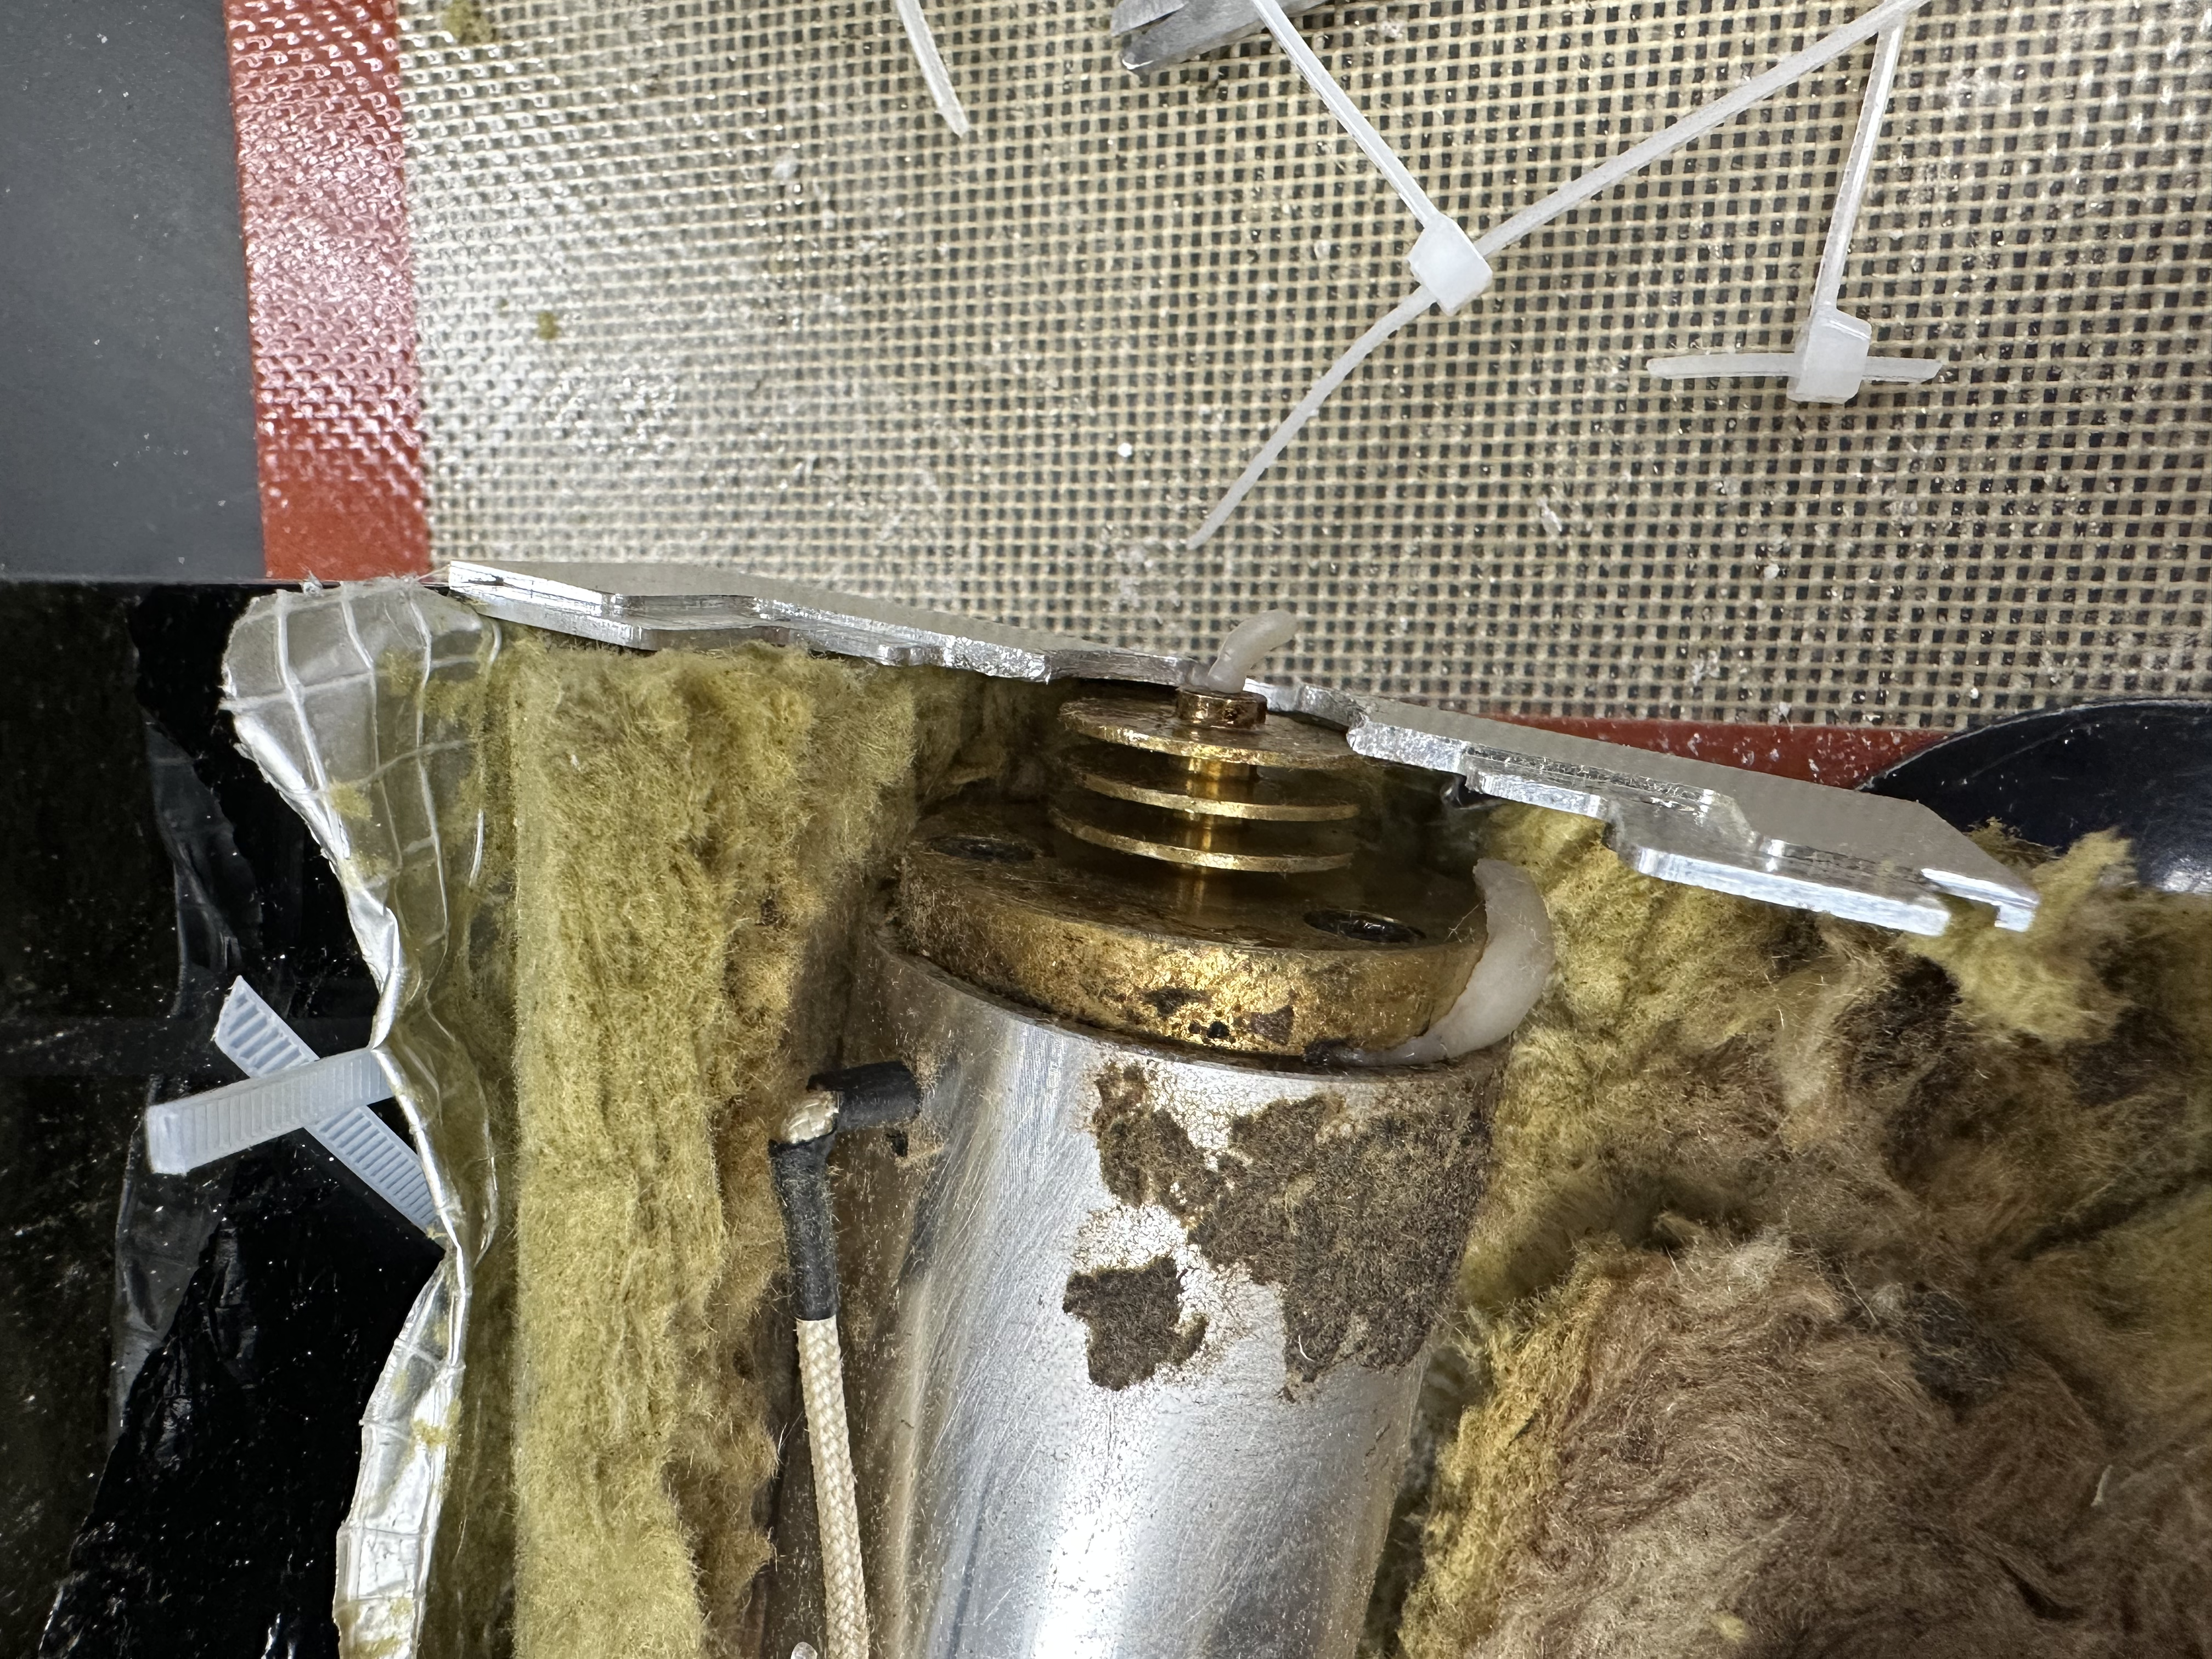
\includegraphics[width=0.5\linewidth]{../figs/methodology/plclExtrusions/pelletExtrusions/felfilEvo/broken_o_ring.png}
        \caption{Material seeping from nozzle/barrel interface following full extruder disassembly.}
        \label{fig:methodology:extrudingPLCL:pelletExtrusions:felfilEvo:brokenORing}
\end{figure}

\paragraph*{Initial PLA Testing}

Once the extruder was fully reassembled, it was tested using PLA pellets as this is an initial test extrusion 3Devo recommends~\cite{RefWorks:RefID:396-3devotroubleshooting}.

This extrusion yielded good-quality PLA filament as shown below in Figure~\ref{fig:methodology:extrudingPLCL:pelletExtrusions:felfilEvo:initialPLAFilament}.

\begin{figure}[h!]
        \centering
        \includegraphics[width=0.7\linewidth]{../figs/methodology/plclExtrusions/pelletExtrusions/felfilEvo/initial_PLA_test.png}
        \caption{Initial PLA pellet test with Felfil Evo. Test setup (A) and unspooled output (B).}
        \label{fig:methodology:extrudingPLCL:pelletExtrusions:felfilEvo:initialPLAFilament}
\end{figure}

\subsubsection{Felfil Evo PLCL Extrusion\label{sec:methodology:extrudingPLCL:felfilSystem:felfilEvoPLCL}}

Following the successful PLA pellet-based extrusion on the Felfil Evo (see Section~\ref{sec:methodology:extrudingPLCL:felfilSystem:felfilEvoInitialTesting}), a PLA/PCL extrusion was attempted using the same methodology as the 3Devo PLA/PCL extrusions (see Section~\ref{sec:methodology:extrudingPLCL:pelletExtrusions:usingStarveFeeder:initialPLCLExtrusion}).

The Felfil Evo has one heat zone which was initially set at 170\textcelsius ~and was raised to 170\textcelsius. The screw RPM was set to 4.

Results and discussion of this PLCL extrusion can be found in \fullref{sec:results:extrudingPLCL:pelletExtrusions:felfilEvo:initialPLCL} and ~\fullref{sec:discussion:extrudingPLCL:pelletExtrusions:felfilEvo:initialPLCL} respectively.

\subsubsection{Felfil Evo Hopper Improvements\label{sec:methodology:extrudingPLCL:felfilSystem:felfilEvoHopperImprovements}}

Multiple ideas were brainstormed to insulate the hopper from the extrusion material. Time and cost of materials were prioritized when ranking options. Final options included a rubber or silicone inserted layer or a 3D printed insulator piece.

\paragraph*{Silicone Coating\label{sec:methodology:extrudingPLCL:felfilSystem:felfilEvoHopperImprovements:siliconeCoating}}

Initially, a rubber or silicone coating was explored to act as a barrier between the extruded material and metal wall.

Electronics subject-matter experts across Ohio State University were consulted to see if they have used any similar materials for heat insulation. Multiple potential challenges were presented through these conversations such as the inability of adhesives to withstand high temperatures.

Various materials were researched, regardless, to assess the viability of this option. Some of these materials are shown below in Figure~\ref{fig:methodology:extrudingPLCL:pelletExtrusions:felfilEvo:siliconHopperCoating}

\begin{figure}[h!]
        \centering
        \includegraphics[width=0.7\linewidth]{../figs/methodology/plclExtrusions/pelletExtrusions/felfilEvo/various_rubber_coatings.png}
        \caption{Various rubber insulator materials researched~\cite{RefWorks:RefID:496-silicone,RefWorks:RefID:497-general,RefWorks:RefID:498-silicone,RefWorks:RefID:499-hightemperature}.}
        \label{fig:methodology:extrudingPLCL:pelletExtrusions:felfilEvo:siliconHopperCoating}
\end{figure}

Based on the concerns addressed by subject-matter experts and the potential lead time of ordering materials, a 3D printed approach was prioritized.

\paragraph*{3D Printed Hopper Insert\label{sec:methodology:extrudingPLCL:felfilSystem:felfilEvoHopperImprovements:3dPrintedHopperInsert}}

\hl{STOPPED HERE!}
% a. Created a 3D printed insert to block the heat transfer
% b. Modeled it in SolidWorks after using the existing CAD files to create an assembly of the hopper
% c. Took 5 versions to properly account for the screw (couldn't measure by hand without fully disassembling machine)
% d. Added thickness and slope to address thin insert still getting hot
% i. Add distance between wall and raw materials

\subsubsection{Logging Filament Thickness\label{sec:methodology:extrudingPLCL:felfilSystem:filamentThickness}}

\paragraph*{Need to Log Thickness}
% a. Realized I needed to log thickness data to analyze it like DevoVision does

Following the initial PLCL extrusions on the Felfil system (see ~\fullref{sec:methodology:extrudingPLCL:felfilSystem:felfilEvoPLCL}), it was determined that a system for quantitatively monitoring filament thickness was necessary to properly compare this system to the 3Devo Filament Maker One.

\paragraph*{Accessing Firmware}
% a. Felfil is open source and run on an Arduino Nano
% b. I was able to access the current firmware (V1.8) and modify it
% c. USB-MiniB port is accessible through side of spooler or by taking casing off
The Felfil system is open source and the Spooler+ runs on an Arduino Nano. Thus, it was possible to access the source code and make modifications to the firmware. The version 1.8 source code was downloaded from Felfil's online repository~\cite{RefWorks:RefID:495}.

\paragraph*{Modifying Firmware}
% a. I looked through the firmware and found where the live diameter reading was stored
% b. Started by printing to serial monitor
% c. Created python script to store readings in a csv for easy logging and graphical analysis

The Arduino-based code was read through, and it was noted where filament thickness was calculated and output to the LCD screen.

Initially, the serial monitor was utilized to output filament thickness to the screen. This was more helpful than the initial LCD output as a live list of filament thicknesses could be recorded. However, the Arduino serial monitor does not inherently support large copy/paste, making it difficult to record and analyze the filament thickness across an extended period of time.

\paragraph*{Filament Thickness GUI}

Due to the limitations of the Arduino serial monitor, a python script was developed to export and visually track the filament thickness similarly to DevoVision.

Claude.ai was used to refine this code. A live visual of the filament thickness GUI is shown below in Figure~\ref{fig:methodology:extrudingPLCL:felfilFilamentThicknessGUI}. The final code is included in ~\fullref{chap:appendix:felfilGUICode}.

\begin{figure}[h!]
        \centering
        \includegraphics[width=0.7\linewidth]{../figs/methodology/plclExtrusions/pelletExtrusions/felfilEvo/felfil_filament_thickness_gui.png}
        \caption{Filament thickness GUI. Created with assistance from Claude.ai.}
        \label{fig:methodology:extrudingPLCL:felfilFilamentThicknessGUI}
\end{figure}

\subsubsection{Felfil Shredder\label{sec:methodology:extrudingPLCL:felfilSystem:felfilShredder}}
% a. Started by shredding multiple times until regrind size looked uniform
% b. Downloaded sieve from Felfil to control for size and make sure everything is ~5mm x 5mm
% c. Discovered that medium-thick filament shreds best

\subsubsection{PLCL Extrusions with System Modifications\label{sec:methodology:extrudingPLCL:felfilSystem:extrusionsAfterModifications}}
% Performed 1st and 2nd pass extrusions with the filament thickness monitoring and hopper insulation
% Manually adjusted RPM, fan speed, and heat (see extrusion summary excel sheet)
% Hopper insulator helped with clumping (10/22 #5 extrusion, didn't have to stir pellets or remove clumps at all)
